
%% Requires compilation with XeLaTeX or LuaLaTeX
\documentclass[10pt,xcolor={table,dvipsnames},t]{beamer}
\usetheme{UCBerkeley}

\title[Your Short Title]{COMP8240}
\subtitle{Major Project Proposal Presentation by Group C}
\author{Kuk Kim and Reeba Fatima}
%\institute{Your Faculty/Department}
\date{30 August 2022}

\begin{document}

\begin{frame}
  \titlepage
\end{frame}

%---------------------------------------------------------
% Uncomment these lines for an automatically generated outline.
%\begin{frame}{Summary}
%  \tableofcontents
%\end{frame}

%---------------------------------------------------------  INTRODUCTION SLIDE
\section{Introduction}
\begin{frame}{Introduction}

\begin{itemize}
  \item Default project
  \item Topic: \texttt{fastText Classification}
  \item Paper: 
  \item Author: 
\end{itemize}

\begin{block}{Examples}
Some examples of commonly used commands and features are included, to help you get started.
\end{block}

\end{frame}
%---------------------------------------------------------  Justification for project basis: NOT REQUIRED

%---------------------------------------------------------  Explicit inclusion of unit techniques and tools
\section{Inclusion of unit techniques and tools}
\begin{frame}{Inclusion of unit techniques and tools}

\begin{itemize}
  \item Oracle cloud virtual machine to run fastText code
  \item Github
    \begin{itemize}
        \item Remote repository to store codes
        \item Version control for collaboration between group members
    \end{itemize}
  \item Overleaf
    \begin{itemize}
        \item Generating LaTeX document and presentation slides
    \end{itemize}
  \item Python
    \begin{itemize}
        \item Programming language used to collect raw data
        \item Carry out raw data clean up and pre-processing
        \item Generate new data sets
    \end{itemize}
\end{itemize}

\end{frame}
%---------------------------------------------------------  Replication of original work
\section{Replication of original work}
\begin{frame}{Replication of original work}

    \begin{itemize}
        \item \textbf{fastText}
    \end{itemize}
    
    \textit{fastText} is a text classifier program to solve text classification problems such as spam detection, sentiment analysis or smart replies. \newline
    
    \textit{fastText} program is donwdloaded and executed in Oracle Cloud Virtual Machine environment. \newline

\end{frame}
%---------------------------------------------------------  Replication of original work cont.
\section{Replication of original work 2}
\begin{frame}{Replication of original work cont.}

    \begin{itemize}
        \item \textbf{fastText}
    \end{itemize}

    We are exploring the following aspects of \textit{fastText}:
    \begin{itemize}
        \item using different hyper-parameters
            \begin{itemize}
                \item \textbf{number of epochs}: number of times each examples is seen
                \item \textbf{learning rate}: how much model changes after processing each example
            \end{itemize}
        \item using word \textbf{bigrams} as opposed to unigrams
            \begin{itemize}
                \item especially important for classification problems where word order is important
            \end{itemize}
        \item using \textbf{hierarchical softmax} as opposed to regular softmax, i.e. \textit{Huffman tree}
            \begin{itemize}
                \item loss function that approximates the softmax with a much faster computation
            \end{itemize}
        \item using pretrained embeddings
    \end{itemize}

\end{frame}
%---------------------------------------------------------  New data #1
\section{New data exploration 1}
\begin{frame}{New data exploration}

New set of labelled data is required to train supervised classifier.
\newline
    \begin{itemize}
        \item Dataset \#1
            \begin{itemize}
                \item Data is collected from Twitter, total of 15,000 Tweets
                \item Uses Python's \textit{}{tweepy} library to gather Tweets through \texttt{Tweeter API v3.0}
                \item \textit{Condition}: Retrieve TOP 100 most trending hashtags and collect 15000  Tweets associated
                \item Pre-process raw data to remove upper case letters, URLs, and punctuations to improve the performance of model
                \item Generate multi-labelled data
                    \begin{itemize}
                        \item Sample: \texttt{\_label\_hashtag\#1 \_label\_hashtag\#2 Tweet text} 
                    \end{itemize}
            \end{itemize}
    \end{itemize}

\end{frame}

%---------------------------------------------------------  New data #1 cont.
\section{New data exploration 2}
\begin{frame}{New data exploration cont.}

    \begin{itemize}
        \item Dataset \#1
            \begin{itemize}
                \item Aspects of the tutorial intending to investigate on new datasets
                 \item Investigate predicted hashtags outcome to analyse if fastText can still be good fit for my use case.
                    Automatically recognise the hashtag of Tweet mention like text. Topic recognition
                \item 
            \end{itemize}
    \end{itemize}

\end{frame}
%---------------------------------------------------------  New data #2
\section{New data exploration 3}
\begin{frame}{New data exploration cont.}

New dataset description

    \begin{itemize}
        \item Dataset \#2
            \begin{itemize}
                \item 
                \item 
                \item 
                \item 
            \end{itemize}
        \item 
            \begin{itemize}
                \item 
            \end{itemize}
        \item
            \begin{itemize}
                \item
            \end{itemize}
    \end{itemize}
    
\end{frame}
%---------------------------------------------------------  Empty slide
\section{Empty slide}
\begin{frame}{Empty slide}

    
\end{frame}
%---------------------------------------------------------  Empty slide
\section{Empty slide}
\begin{frame}{Empty slide}

    
\end{frame}
%---------------------------------------------------------  Empty slide
\section{Empty slide}
\begin{frame}{Empty slide}

    
\end{frame}
%---------------------------------------------------------

\section{Some \LaTeX{} Examples}

\subsection{Mathematics}

\begin{frame}{Readable Mathematics 42}

Let $X_1, X_2, \ldots, X_n$ be a sequence of independent and identically distributed random variables with $\text{E}[X_i] = \mu$ and $\text{Var}[X_i] = \sigma^2 < \infty$, and let
$$S_n = \frac{X_1 + X_2 + \cdots + X_n}{n}
      = \frac{1}{n}\sum_{i}^{n} X_i$$
denote their mean. Then as $n$ approaches infinity, the random variables $\sqrt{n}(S_n - \mu)$ converge in distribution to a normal $\mathcal{N}(0, \sigma^2)$.

\end{frame}
%---------------------------------------------------------

\subsection{Tables and Figures}

\smallframetitle

\begin{frame}{Tables and Figures}

\begin{itemize}
\item Use \texttt{tabular} for basic tables --- see Table~\ref{tab:widgets}, for example.
\item You can upload a figure (JPEG, PNG or PDF) using the files menu. 
\item To include it in your document, use the \texttt{includegraphics} command (see the comment below in the source code).
\end{itemize}

\begin{table}
\centering
\begin{tabular}{l r}
\tableheadrow
\tableheadcol{Item} & \tableheadcol{Quantity} \\
Widgets & 42 \\
Gadgets & 13
\end{tabular}
\caption{\label{tab:widgets}An example table.}
\end{table}

\end{frame}
%---------------------------------------------------------
\begin{frame}
\frametitle{Figure Example}

Commands to include a figure:

\begin{figure}
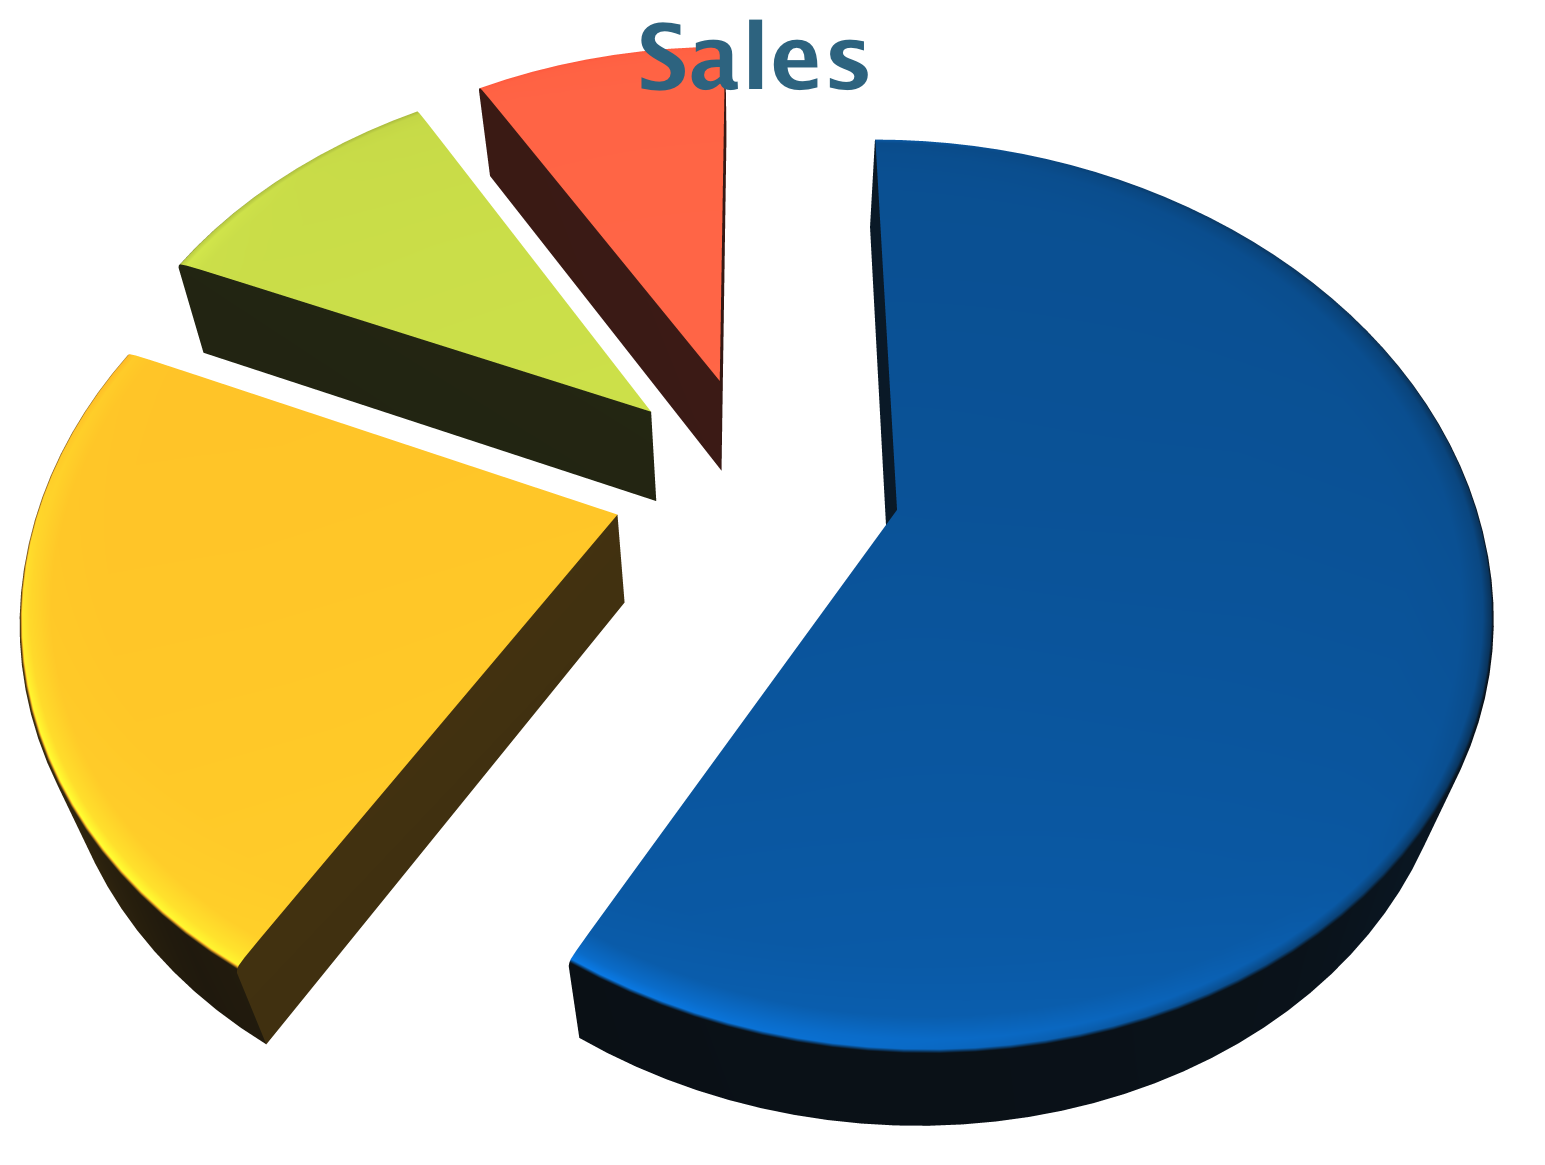
\includegraphics[width=0.4\textwidth]{chart}
\caption{\label{fig:your-figure}Caption goes here.}
\end{figure}
\end{frame}
%---------------------------------------------------------
\begin{frame}
\frametitle{Text in Two Columns}

\begin{columns}[T]

\begin{column}{0.48\textwidth}
\small
Lorem ipsum dolor sit amet, consectetur adipiscing elit. Fusce sit amet massa in dolor pellentesque tempor. Integer nunc. 
\end{column}

\begin{column}{0.48\textwidth}
\begin{itemize}
\item First bullet goes here
  \begin{itemize}
  \item Secondary bullet goes here
    \begin{itemize}
    \item Tertiary bullet goes here
    \end{itemize}
  \end{itemize}
\end{itemize}
\end{column}

\end{columns}
\end{frame}
%---------------------------------------------------------

\end{document}
